\newpage
\section{Agenti basati su coscenza}
Abbiamo già visto agenti con stato e con obiettivo in mondi osservabili con stati atomici e azioni descrivibili
in maniera semplice, mettendo enfasi sul processo di ricerca.\\\\
Ora andremo ad parlare di come migliorare le \textbf{capacità di ragionamento} degli agenti,
dotandoli di rappresentazioni di mondi complessi e astratti, non descrivibili semplicemente.
Agenti \textbf{basati su conoscenza}, dotati di una KB (\textbf{Knowledge Base}) con conoscenza espressa in maniera esplicita e dichiarativa.
\subsection{Introduzione}
La maggior parte dei problemi di I.A. sono “knowledge intensive”. Il mondo è tipicamente complesso: ci serve una rappresentazione
\textbf{parziale} e \textbf{incompleta} (un’astrazione) del mondo funzionale agli scopi dell’agente. Per ambienti parzialmente osservabili e complessi ci servono
linguaggi di rappresentazione della conoscenza più espressivi e capacità inferenziali. La conoscenza può essere codificata a mano ma anche estratta dai
testi o appresa dall’esperienza o estratta/elicitata dagli esperti.\\\\
La KB racchiude tutta la conoscenza necessaria a decidere l’azione da compiere in forma \textbf{dichiarativa}.
Un agente basato su conoscenza può essere costruito dicendogli (TELL) ciò che deve sapere. SI inizia con una base di conoscneza vuota
si aggiungono progressivamente formule alla base di conoscneza, una alla volta.\\\\
L’alternativa (approccio procedurale) è scrivere un programma che implementa il processo decisionale, una
volta per tutte. Un agente KB è più flessibile: più semplice acquisire conoscenza incrementalmente e modificare il
comportamento con l’esperienza.
\begin{example}
    Il mondo del Wumpus. Il mondo del Wumpus è una caverna fatta di stanze connesse tra di loro da
    passaggi. Il wumpus è una bestia puzzolente che mangia chiunque entri nella stanza in
    cui si trova. 
    \begin{figure}[h!]
        \centering
        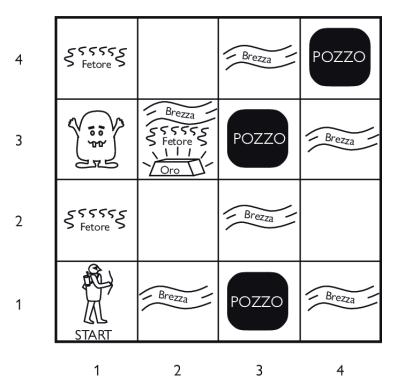
\includegraphics[width=0.4\textwidth]{images/esempio-wumpus.png}
    \end{figure}
    Il wumpus può essere ucciso dall’agente, che ha solo una freccia a disposizione.
    \begin{itemize}
        \item Ci sono stanze con dei pozzi: se l’agente entra in una di queste stanze cade nel pozzo e muore. Il Wumpus non muore nel pozzo.
        \item In una delle stanze si trova l’oro e l’obiettivo dell’agente è di trovare l’oro e tornare a casa con l’oro, sano e salvo.
        \item L’agente non conosce l’ambiente, né la sua locazione. Solo all’inizio sa dove si trova (in [1,1]).
    \end{itemize}
    Abbiamo poi delle misure di prestazioni:
    \begin{itemize}
        \item +1000 se trova l'oro, trona in [1,1] ed esce.
        \item -1000 se muore.
        \item -1 per ogni azione.
        \item -10 se usa la freccia.
    \end{itemize}
    L'\textbf{ambiente} è strutturato in una griglia 4 x 4 di stanze, circondata da pareti di delimitazione.
    L’agente comincia sempre dalla posizione [1,1], rivolto verso est (dx) ([1,1] è safe).
    Le posizioni dell’oro e del Wumpus sono scelte casualmente tra tutti I riquadri tranne quello iniziale.
    Tutti I riquadri (tranne quello iniziale) hanno una probabilita’ 0.2 di contenere un pozzo.\\\\
    Le \textbf{azioni} disponibili sono: avanti, a destra di 90°, a sinistra di 90°, afferra un oggetto, scaglia la freccia (solo una), esce.
    Le cose che vengono \textbf{percepite} (sesori) sono:
    \begin{itemize}
        \item fetore nelle caselle adiacenti al Wumpus.
        \item brezza nelle caselle adiacenti ai pozzi.
        \item Luccichio nelle caselle con l'oro.
        \item Bump se sbatte in un muto
        \item Urlo se il wumpus viene ucciso.
        \item L'agente NON percepisce la sua locaizone.
    \end{itemize}
\end{example}

\begin{figure}[h!]
    \begin{subfigure}{0.24\textwidth}
        \centering
        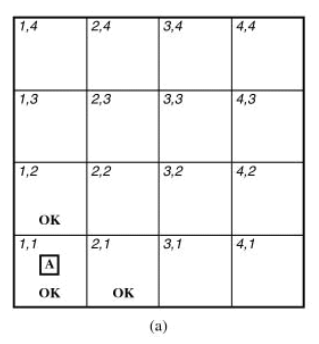
\includegraphics[width=\textwidth]{images/ess-wumpus-scenario-1.png}
        \caption{Scenario 1}
    \end{subfigure}
    \begin{subfigure}{0.24\textwidth}
        \centering
        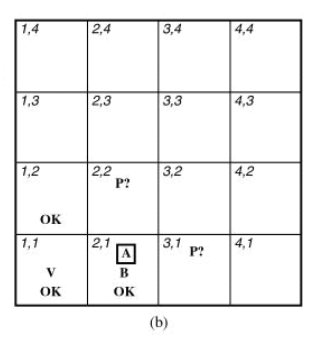
\includegraphics[width=\textwidth]{images/ess-wumpus-scenario-2.png}
        \caption{Scenario 2}
    \end{subfigure}
    \begin{subfigure}{0.24\textwidth}
        \centering
        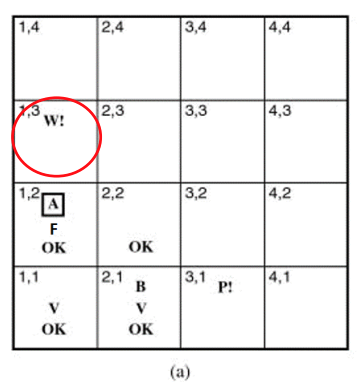
\includegraphics[width=\textwidth]{images/ess-wumpus-scenario-3.png}
        \caption{Scenario 3}
    \end{subfigure}
    \begin{subfigure}{0.24\textwidth}
        \centering
        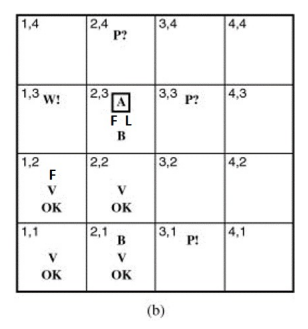
\includegraphics[width=\textwidth]{images/ess-wumpus-scenario-4.png}
        \caption{Scenario 4}
    \end{subfigure}
\end{figure}
\begin{enumerate}
    \item La percesione sono quintuple: [fetore, brezza, luccichio, bump, urlo].\\
    Percesione [1,1] = [none, none,none, none], non essendoci ne brezza ne fetore in [1,1] allora
    [1,2] e [2,1] sono sicure (OK), l'agente decide di spostarsi in [2,1].
    \item Percezione in [2,1] [none,Brezza,none,none,none].\\
    L’agente percepisce una Brezza. Quindi c’è un pozzo in [2,2] o [3,1] (P?). L’agente torna in [1,1] e poi si
    sposta in [1,2].
    \item Percezione in [1,2]: [Fetore,none,none,none,none]\\
    Il Wumpus non può essere in [1,1] (safe per definizione), né in [2,2] (altrimenti avrebbe percepito Fetore anche in [2,1]). Quindi è in [1,3].\\
    Siccome non c’è Brezza in [1,2], [2,2] è OK e ci deve essere un Pozzo in [3,1].
    \item L’agente si sposta in [2,2] e poi in [2,3]. Percezione in [2,3] [Fetore, Brezza, Luccichio, none,none].\\
    Percepisce un Luccichio, afferra l’Oro e torna sui suoi passi, percorrendo caselle OK.
\end{enumerate}

\newpage
\subsection{Agenti basati sulla conoscenza}
Un agente basato su conoscenza mantiene una \textbf{base di conoscenza} (KB): un insieme di \textbf{enunciati} (formule) espressi in un
linguaggio di rappresentazione. Interagisce con la KB mediante una interfaccia funzionale Tell-Ask:
\begin{itemize}
    \item Tell: per aggiungere nuovi enunciati a KB.
    \item Ask: per interrogare la KB.
    \item Retract: per eliminare enunciati.
\end{itemize}
Gli enunciati nella KB rappresentano le \textbf{opinioni/credenze dell’agente}. Le risposte $\alpha$ devono
essere tali che $\alpha$ \textbf{discende necessariamente} dalla KB.\\\\
Il problema: data una base di conoscenza KB, contenente una rappresentazione dei fatti che si
\textbf{ritengono veri}, come dedurre che un certo fatto a è vero di conseguenza?
$$KB |= \alpha \hspace{15pt}\text{conseguenza logica}$$
\begin{lstlisting}
    //Prende in input una percezione e restituisce un azione
    function Agente-KB (percezione) returns un azione
        //Mantiene in memoria una base di conoscenza KB che puo contenere una conoscenza iniziale.
        persistent: KB, una base di conoscenza
        t, un contatore, inizialmente a 0, che indica il tempo

        // Comunica la percezione all KB
        TELL(KB, Costruisci-Formula-Percezione(percezione, t ))

        // Chiede alla KB quale azioni deve compiere
        azione <- ASK(KB, Costruisci-Query-Azione( t ))

        // Comunica alla KB che l azione e stata compiuta al tempo t
        TELL(KB, Costruisci-Formula-Azione(azione, t ))
        t <- t + 1
        return azione
\end{lstlisting}
Base di conoscenza vs base di dati:
\begin{itemize}
    \item \textbf{base di dati}: solo fatti specifici, solo recupero (retrieval).
    \item \textbf{Base di conoscenza}: una rappresentazione esplicita, parziale e compatta, in un linguagio simbolico, che contiene:
    fatti di timpo specifico (casella [1,1] ok, c'è un posso in [3,1]), fatti di tipo generale, o regole (c'è brezza nella caselle adiacenti ai pozzi).
\end{itemize}
Qullo che caratterizza una KB è la capacità inferenziale, derivare nuovi fatti da quelli memorizzati esplicitamente (es. c'è un pozzo in [3,1] il wumpus è in [1,3]).\\
Sfortunatamente pià il linguaggio è \textbf{espressivo}, meno \textbf{efficiente} è il meccanismo inferenziale. § Il problema ‘fondamentale’ in R.C. è trovare il giusto
compromesso tra: \textbf{espressività} del linguaggio di rappresentazione, \textbf{complessità} del meccanismo inferenziale.\\
Questi due obiettivi sono in contrasto e si tratta di mediare tra queste due esisgenze.

\subsection{Logica}
Le basi di conoscenza sono costituite da enunciati (formule). Le formule sono espresse secondo le regole della sintassi,
che specifica quali di esse sono “ben formate”. La semantica di una formula esprime il “significato” della
formula. Un modello e’ una configurazione dei valori di verità che si possono assegnare alle variabili convolte in una formula.\\\\
Un formalismo per la rappresentazione della conoscneza ha tre componenti:
\begin{enumerate}
    \item Una \textbf{sintassi}: un linguaggio composto da un vocabolario e regole per la formazione delle frasi (enuciati, formule).
    \item Una \textbf{semantica}: stabilisce una corrisondenza tra gli enunciati e i fatti del mondo; se un agente ha un enunciato $\alpha$ nella KB, crede ch eil fatto corrispondente sia vero nel mondo.
    \item Un \textbf{meccanismo inferenziale} (codificato o meno tramite regole di inferenza come nella logica) che ci consente di inferire nuovi fatti.
\end{enumerate}
\begin{definition}[Semantica]
    La semantica specifica le regole usate per determinare il valore di verità di una formula nei confronti di un particolare modello.
\end{definition}
Nella logica proposizionale, un modello specifica il valore di verità (True o False) di ogni simbolo proposizionale.
\begin{figure}[h!]
    \centering
    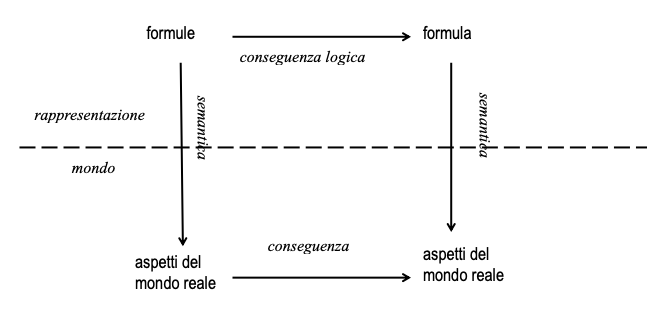
\includegraphics[width=0.65\textwidth]{images/rappresentazione_e_mondo.png}
\end{figure}

\hspace{-15pt}Le formule sono configurazioni fisiche dell’agente. 
Il ragionamento e’ il processo di costruzione di nuove configurazioni partendo dale vecchie. 
Il ragionamento logico dovrebbe assicurare che le nuove configurazioni rappresentino aspetti del mondo che sono effettive conseguenze degli aspetti delmondo rappresentati dale vecchie configurazioni
\newpage
\section{Logica Proposizionale}
\subsection{Sintassi}
\begin{definition}[Sintassi]
    La sintassi definisce quali sono le frasi leggittime (ben formate) del linguaggio.
    \begin{equation*}
        \begin{split}
            formula & \longrightarrow formulaAtomica \:\: | \:\: formula complessa \\
            formulaAtomica & \longrightarrow True \:\: | \:\: False \:\: | \:\: simbolo \\
            simbolo & \longrightarrow P \:\: | \:\: Q \:\: | \:\: R \:\:| \:\: \dots\\
            formulaComplessa & \longrightarrow \lnot formula \text{ not (negazione)}\\
            & | \:\: (formula \land formula) \text{ and (congiuzione )}\\
            & | \:\: (formula \lor formula) \text{ or (disgiunzione)}\\
            & | \:\: (formula \Rightarrow formula) \text{ implicazione}\\
            & | \:\: (formula \Leftrightarrow formula) \text{ se e solo se}\\
        \end{split}
    \end{equation*}
\end{definition}

\begin{example}
    $((A \land B) \Rightarrow C)$.
    Possiamo oettere le parentesi assumendo questa precedenza tra gli operatori:
    $$\lnot \:\: > \:\: \land \:\: > \:\: \lor \:\: > \:\: \Rightarrow, \Leftrightarrow$$
    $\lnot P \land Q \lor R \Rightarrow S$ è la stessa cosa di $(((\lnot P) \lor (Q \land R)) \Rightarrow)$. Per esempio
    dal mondo del Wumpus $P_{1,1}$ c'è il posso in $[1,1]$, $W_{2,3}$ il wumpus è in $[2,3]$.
\end{example}

\subsection{Semantica}
\begin{definition}
    La semantica specifica le regole usate per determinare il valore di verità di una formula nei confronti di un particolare modello.
\end{definition}
\hspace{-15pt}Nella logica proposizionale, un modello specifica il
valore di verità (True o False) di ogni simbolo proposizionale.\\\\
La semantica ha a che fare col significato delle frasi: definisce se un enunciato
è vero o falso rispetto a una interpretazione (mondo possibile). Una interpretazione definisce un valore di verità per tutti i simboli proposizionali.
\begin{example}
    $\{P_{1,1} \text{ vero, } P_{1,2} \text{ false, } W_{w,3} \text{ vero}\}$
\end{example}
\subsubsection{Semantica composizionale}
Il significato di una frase è determinato dal significato dei suoi componenti, a partire dalle frasi atomiche (i simboli proposizionali).
\begin{figure}[h!]
    \centering
    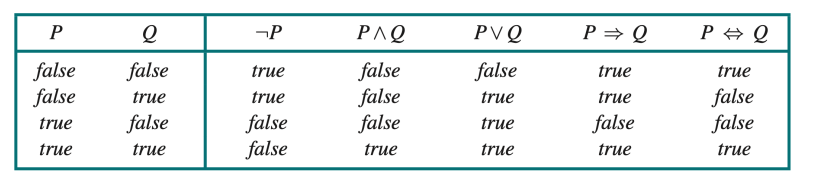
\includegraphics[width=0.65\textwidth]{images/tavola-vertià.png}
\end{figure}

\hspace{-15pt}La logica proposizionale non richiede alcuna relazione di causalità 
Per esempio per $P \Rightarrow Q$ in effetti significa che “Se P è vero, allora sostengo che lo è anche Q. Se P è falso, allora non faccio alcuna asserzione”\\\\
Una formula $\alpha$ è conseguenza logica di un insieme di
formule KB se e solo se in ogni modello di KB, anche $\alpha$
è vera ($KB \models \alpha$).\\\\
Indicando con M(KB) i modelli dell’insieme di formule
in KB e con M($\alpha$) l’insieme delle interpretazioni che
rendono $\alpha$ vera (i modelli di $\alpha$)
$$KB \models \alpha \:\: sse \:\: M(KB) \subseteq M(\alpha)$$

\subsubsection{Model checking}
Un modo (semplice) per determinare la conseguenza logica. Si enumerano i modelli. 
Si mostra che la formula $\alpha$ deve valere in tutti i modelli in cui è vera la KB.
Si usa per eseguire “inferenze logiche”, derivare una conclusione che segue logicamente da una KB
\begin{example}
    La KB iniziale $KB_0$ è costituita dalle regole generali del WW e deal fatto che la casella iniziale è safe per definizione.
    $$\lnot W_{1,1} \:\: \lnot P_{1,1} \text{ la casella iniziale è safe}$$
    Esempio di regole generate: 
    $$B_{2,1} \Leftrightarrow (P_{1,1} \lor P_{2,2} \lor P_{3,1}) \hspace{15pt} B_{1,1} \Leftrightarrow (P_{1,2} \land P_{2,1})$$
    L’agente non ha percepito nulla in [1,1] e si è spostato in [2,1] dove ha percepito una Brezza. $KB_1$ a questo punto è $KB_0$
    più i fatti corrispondenti alle percezioni $$KB_0 \cup \{\lnot B_{1,1}, B_{2,1}, \lnot F_{1,1}, \lnot F_{2,1}, \cdots\}$$
    Domandiamoci se le stanze adiacenti non contengono pozzi
    $$KB_1 \models \lnot P_{1,2} \hspace{10pt} KB_1 \models \lnot P_{2,2} \hspace{10pt} KB_1 \models \lnot P_{3,1}$$
    Cosa sappiamo all'inizio (quindi cosa c'è in $KB_0$):
    \begin{itemize}
        \item In [1,1] non ci sono pozzi: $R1: \lnot P_{1,1}$
        \item In una stanza si percepisce brezza se e solo se c’è un pozzo in una stanza adiacente (di seguito solo per le posizioni rilevanti):
        $$R2: B_{1,1} \Leftrightarrow (P_{1,2} \lor P_{2,1}) \hspace{15pt} R3: B_{2,1} \Leftrightarrow (P_{1,1} \lor P_{2,2} \lor P_{3,1})$$
    \end{itemize}
    Cosa sappiamo in base alle percezioni (cosa aggiungiamo alla KB):
    \begin{itemize}
        \item Non c'è brezza in [1,1]: $R4: \lnot B_{1,1}$
        \item C'è brezza in [2,1]: $R5: B_{2,1}$
    \end{itemize}
    \begin{figure}[h!]
        \centering
        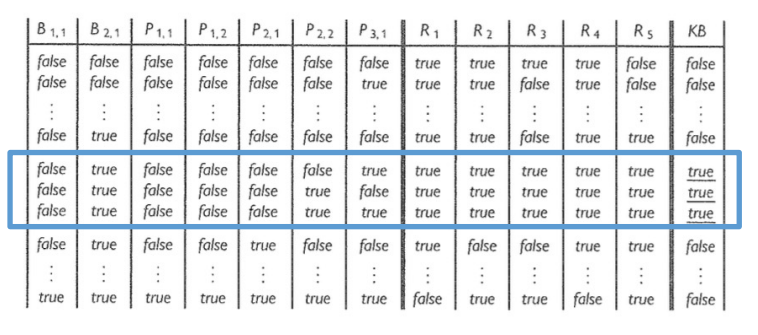
\includegraphics[width=0.5\textwidth]{images/wumpus-logica-prop.png}
    \end{figure}
    Considerando solo l’esistenza di pozzi nelle 3 caselle $P_{1,2}, P_{2,2}, P_{3,1}$ ci sono
    $2^3 = 8$ possibili interpretazioni o mondi possibili.
    \begin{figure}[h!]
        \centering
        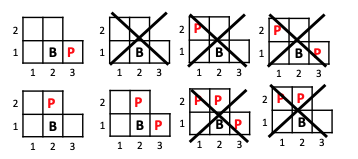
\includegraphics[width=0.5\textwidth]{images/possibili-finali-ess-wumpus-log-prop.png}
    \end{figure}
    $$KB_1 \models \lnot P_{1,2} \hspace{15pt} KB_1 \lnot P_{2,2} \lor P_{3,1} \text{ possiamo conclude che } \lnot P_{2,2} e \lnot P_{3,1} (\text{ne su }P_{2,2} \:e\: P_{3,1} \cdots)$$
\end{example}
